\documentclass[11pt,dvipdfm]{article}
%\documentclass[11pt]{article}
\usepackage{deauthor,times,graphicx}
\usepackage{subfig}
\usepackage{xspace}

\newcommand{\systemname}{\textsc{LedgerBench}\xspace}

%\graphicspath{{authorname/}}

\begin{document}

\title{\systemname: A Framework for Benchmarking Ledger Databases}

\author{
Meihui Zhang \\
Beijing Institute of Technology \\
meihui\_zhang@bit.edu.cn \\
\and
Cong Yue \\
National University of Singapore \\
yuecong@comp.nus.edu.sg \\
\and
Changhao Zhu \\
Beijing Institute of Technology \\
zhuchanghao@bit.edu.cn \\
\and
Ziyue Zhong \\
Beijing Institute of Technology \\
ziyue\_zhong@bit.edu.cn \\
}

\maketitle

\begin{abstract}
Ledger databases protect the integrity of data, history and query results. However, existing ledger databases adopt different design choices, and there is a lack of benchmarking tools to evaluate them comprehensively. Therefore, it is unclear how each design choice performs and it is difficult for users to choose a system that is appropriate for their use case in practice. 
In this paper, we first conduct a survey on the designs of existing systems. 
We categorize the design of ledger database into four components and discuss the design choices of each component. 
Based on the study,
we then outline \systemname, a benchmarking framework for ledger databases, for 
both macro- and micro-benchmarking.
To evaluate the system performance of ledger databases, \systemname provides macro-benchmarks consisting of verification-aware workloads adapted from Smallbank.
To evaluate the performance of each component of a system, it provides micro-benchmarks with respect to verification, verification delay, auditing and storage.
Lastly, we conduct comprehensive experiments on existing ledger databases. 
From the results, we observe that updating the ledger structure and verification is the main bottleneck of ledger databases. The cost can however be significantly reduced by adopting deferred verification and carefully crafted asynchronous ledger update functions that enforce minimum locking. 
\end{abstract}

\section{Introduction}

With the extensive application of cloud computing, outsourced databases and collaborative applications involving multiple parties, users of applications are exposed to various threats caused by the malicious behaviours of outside adversaries and untrusted third-party service providers. There is an increasing demand to protect data security.

In recent years, the ledger database is gaining attention in protecting the integrity of data, history and query results. 
It maintains data or log in the form of append-only ledger, which can generate proofs for users to verify the integrity. Compared to conventional databases, a ledger database has several advantages. 1) It provides efficient verification. The users only need to maintain a cryptographic hash, called digest of the ledger, and integrity check can be performed by comparing the digest against the reproduced hash computed from the proof. 2) It reduces the surface of misbehavior. Since the ledger is immutable, all historical data is protected by the digest. Adversaries cannot tamper with the history without changing the hashes. 3) It can be publicly verified. Everyone can verify the integrity of the data or the log with the ledger. Compared to blockchains, ledger databases offer high performance without the performance bottleneck at consensus layer. Ledger databases are therefore suitable for maintaining financial transactions, logistic orders, healthcare data, etc., where the integrity of data evolution history and proof of data lineage are important.

There are several types of systems that expose ledger APIs, i.e., the system maintains the data and full history in an append-only hash protected authenticated data structure, and can generate proof of each read, update, insert and delete operation to verify the integrity. 
Recently, a bunch of commercial ledger databases has been offered by major service providers, e.g., QLDB \cite{qldb}, LedgerDB \cite{ledgerdb}, and SQL Ledger \cite{sqlledger}. The systems build Merkle tree variances over the transaction logs, and data in the transaction logs are materialized to index structures with meta-information of the log entry. Hence, all queried data can be verified using the log.
Another type of systems is certificate transparency \cite{ct, coniks, merkle2, ect}, where public keys and certificates are protected by Merkle tree variances. Consistency checks can be performed using Merkle proof. 
In addition, blockchains \cite{hyperledger, ethereum, quorum} also expose ledger API. The systems maintain a sequence of hash-chained blocks, and the integrity is guaranteed by replicating the blocks using a byzantine fault tolerant protocol \cite{pbft}. However, they are not our focus due to having a different threat model and design space, and suffering from low performance.

Despite the development of ledger databases, there is a lack of benchmarking tools to systematically and fairly evaluate existing systems. 
Existing key-value and OLTP workloads are unaware of ledger-related functions such as verification and auditing, and therefore, cannot offer accurate analysis of ledger databases. 
In this paper, we outline \systemname, a benchmarking framework for ledger databases. We first conduct a survey on the designs of existing systems. 
We categorize the design of ledger database into four components, namely ledger structure, query processing, verification, and auditing, and discuss the design choices of each component. 
We then design \systemname to evaluate on all four components with micro-benchmarks and
%\systemname  evaluates
the system performance 
%of ledger databases 
with macro-benchmarks consisting of verification-aware OLTP workloads adapted from Smallbank. 
%It evaluates the performance of each component with the micro-benchmark. 
%%% ooibc: this is repetitive of a sentence above
Lastly, we re-construct existing ledger systems based on our understanding of the systems in a consistent manner.
We subsequently conduct extensive experiments on existing ledger databases to illustrate the strengths and weaknesses of each design and system, which may be useful for the future development of ledger databases.

In summary, we make the following contributions.
\begin{itemize}
\item We outline \systemname, the first benchmark for databases that expose ledger APIs. The benchmark is designed to evaluate the performance on all aspects of a ledger database. 

\item We implement an open source \systemname, which can be used or further developed to evaluate other ledger databases.

\item We conduct an extensive evaluation of re-constructed QLDB \cite{qldb}, LedgerDB \cite{ledgerdb}, and SQL Ledger \cite{sqlledger}. 
%%% ooibc: citation for each
Our results pinpoint the performance bottleneck of existing ledger databases, and show the advantage of various design choices.
\end{itemize}

The remaining of the paper is organized as follows. Section~\ref{sec:ldb} briefly surveys the existing ledger databases. Section~\ref{sec:design} explains the design of \systemname. Section~\ref{sec:exp} presents the performance evaluation of four representative systems using \systemname.
Section~\ref{sec:related} discusses the related work before Section~\ref{sec:conclusion} concludes.

\begin{figure}[t]
    \centering
    \begin{minipage}{0.48\textwidth}
        \centering
        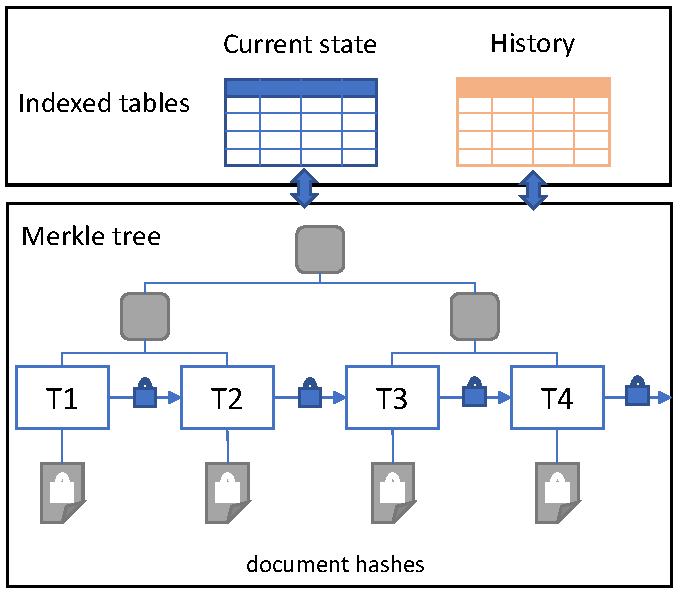
\includegraphics[height=4cm]{figs/arch_qldb.pdf}
        \caption{QLDB architecture}
        \label{fig:qldb}
    \end{minipage}
    \begin{minipage}{0.48\textwidth}
        \centering
        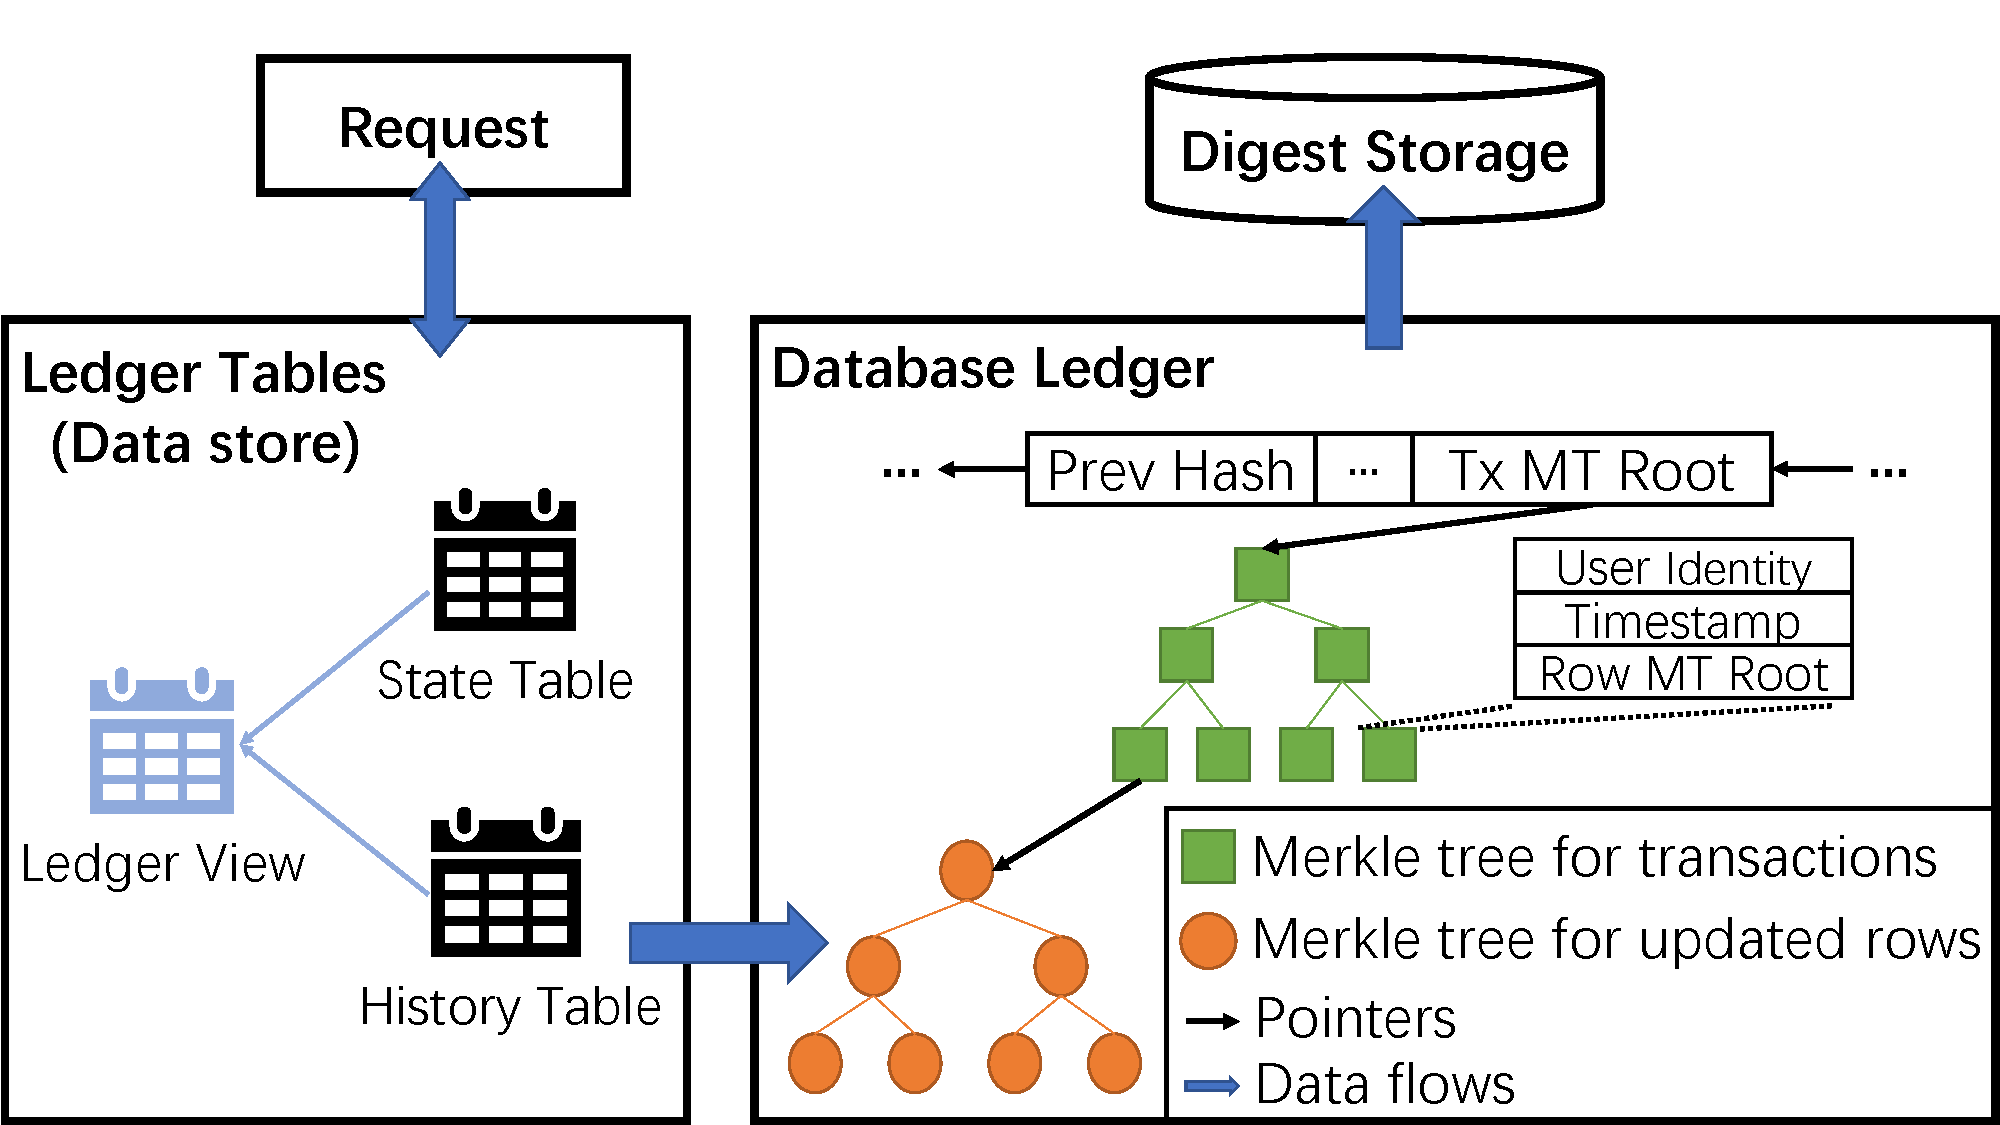
\includegraphics[height=4cm]{figs/arch_sqlledger.pdf}
        \caption{SQL Ledger architecture}
        \label{fig:sqlledger}
    \end{minipage}
\end{figure}

\begin{figure}[t]
    \centering
    \begin{minipage}{0.48\textwidth}
        \centering
        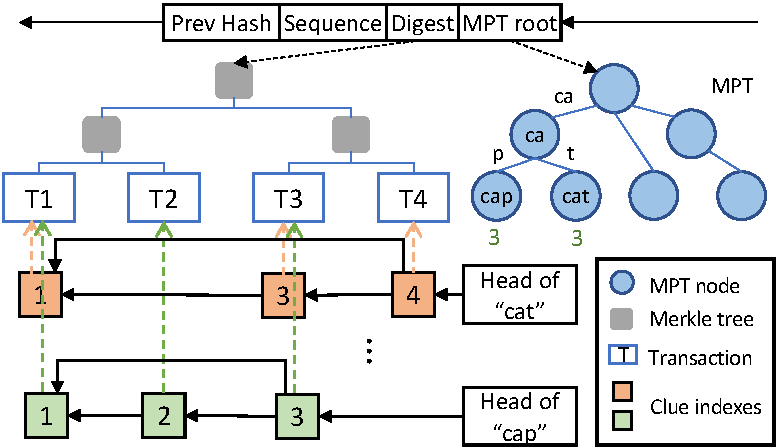
\includegraphics[height=4cm]{figs/arch_ledgerdb.pdf}
        \caption{LedgerDB architecture}
        \label{fig:ledgerdb}
    \end{minipage}
    \begin{minipage}{0.48\textwidth}
        \centering
        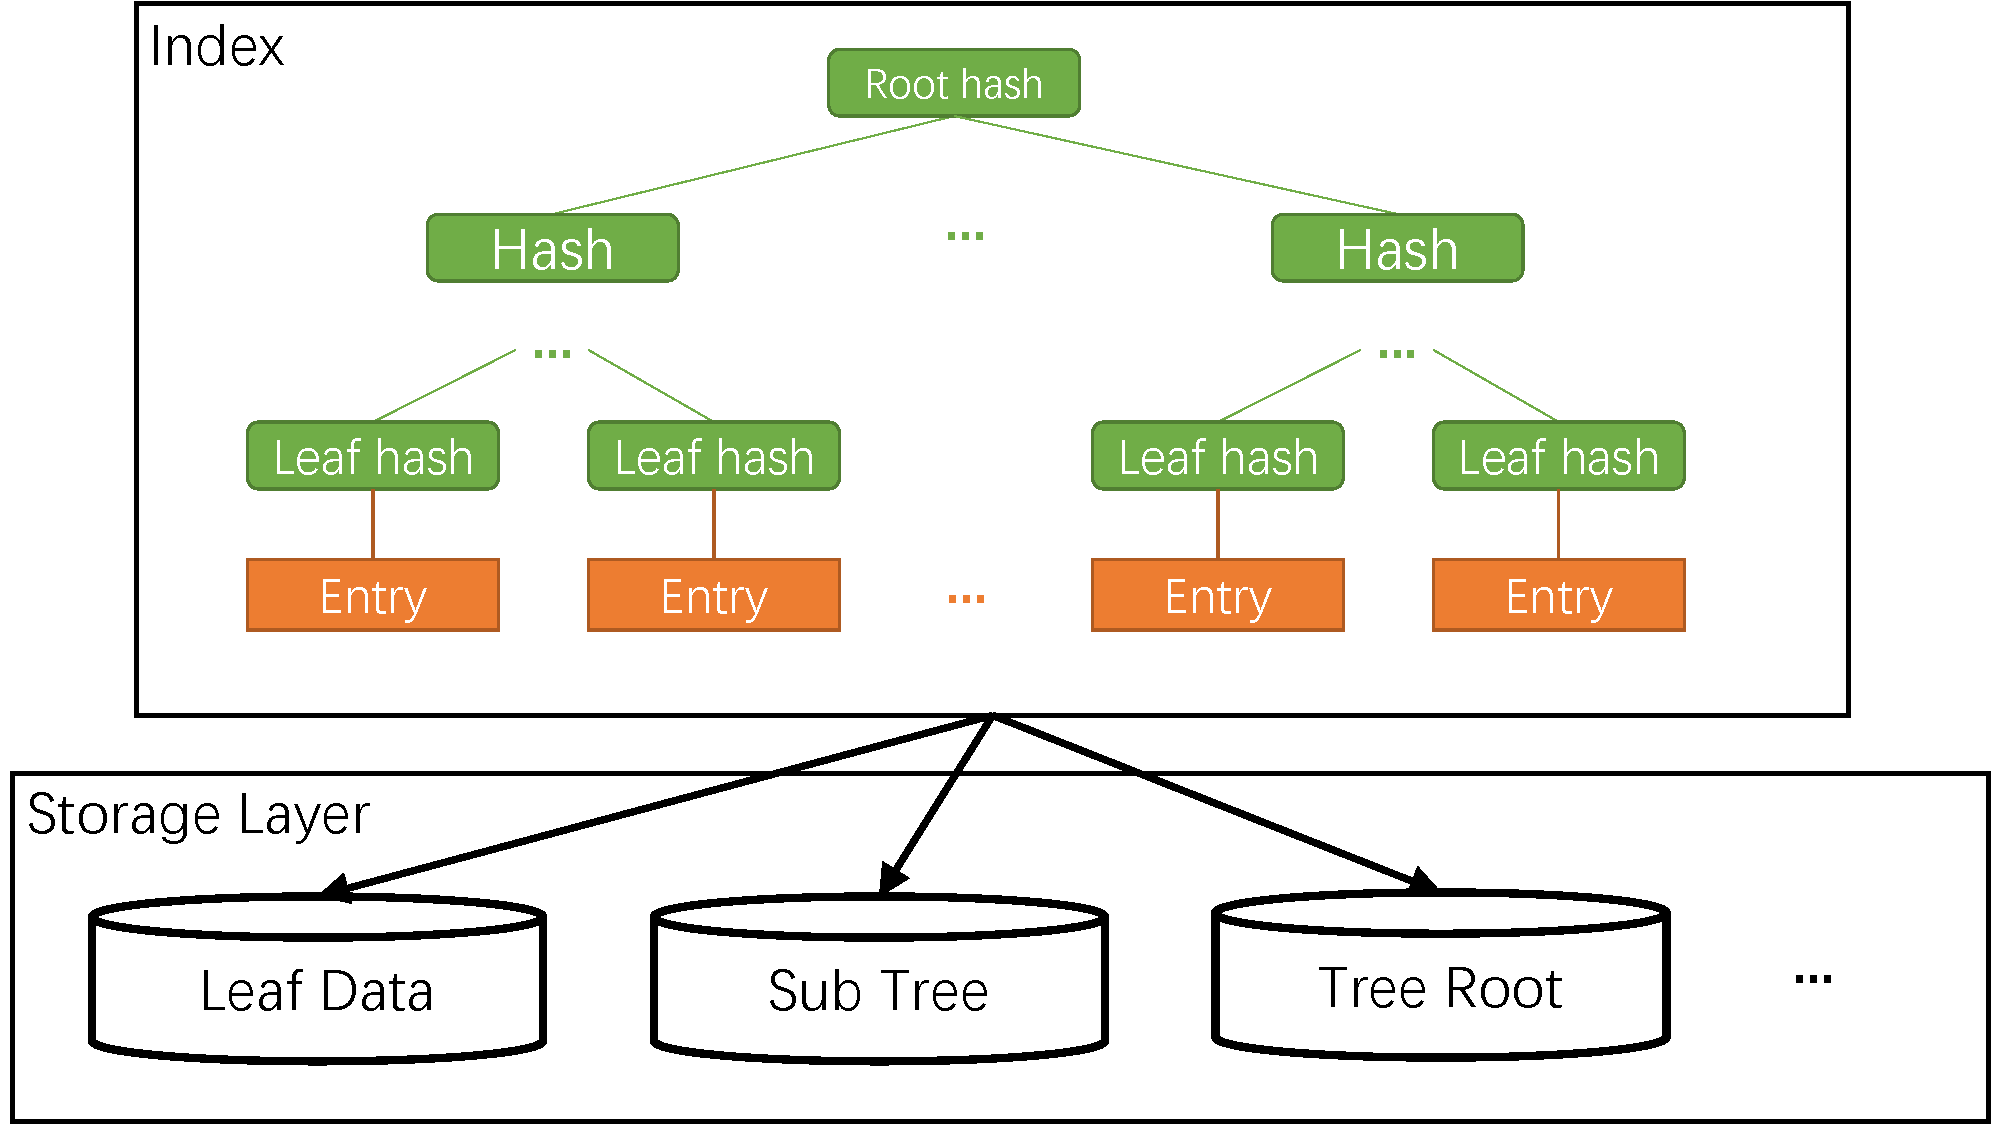
\includegraphics[height=4cm]{figs/arch_trillian.pdf}
        \caption{Trillian architecture}
        \label{fig:trillian}
    \end{minipage}
\end{figure}

\begin{figure}[t]
    \centering
    \begin{minipage}{0.48\textwidth}
        \centering
        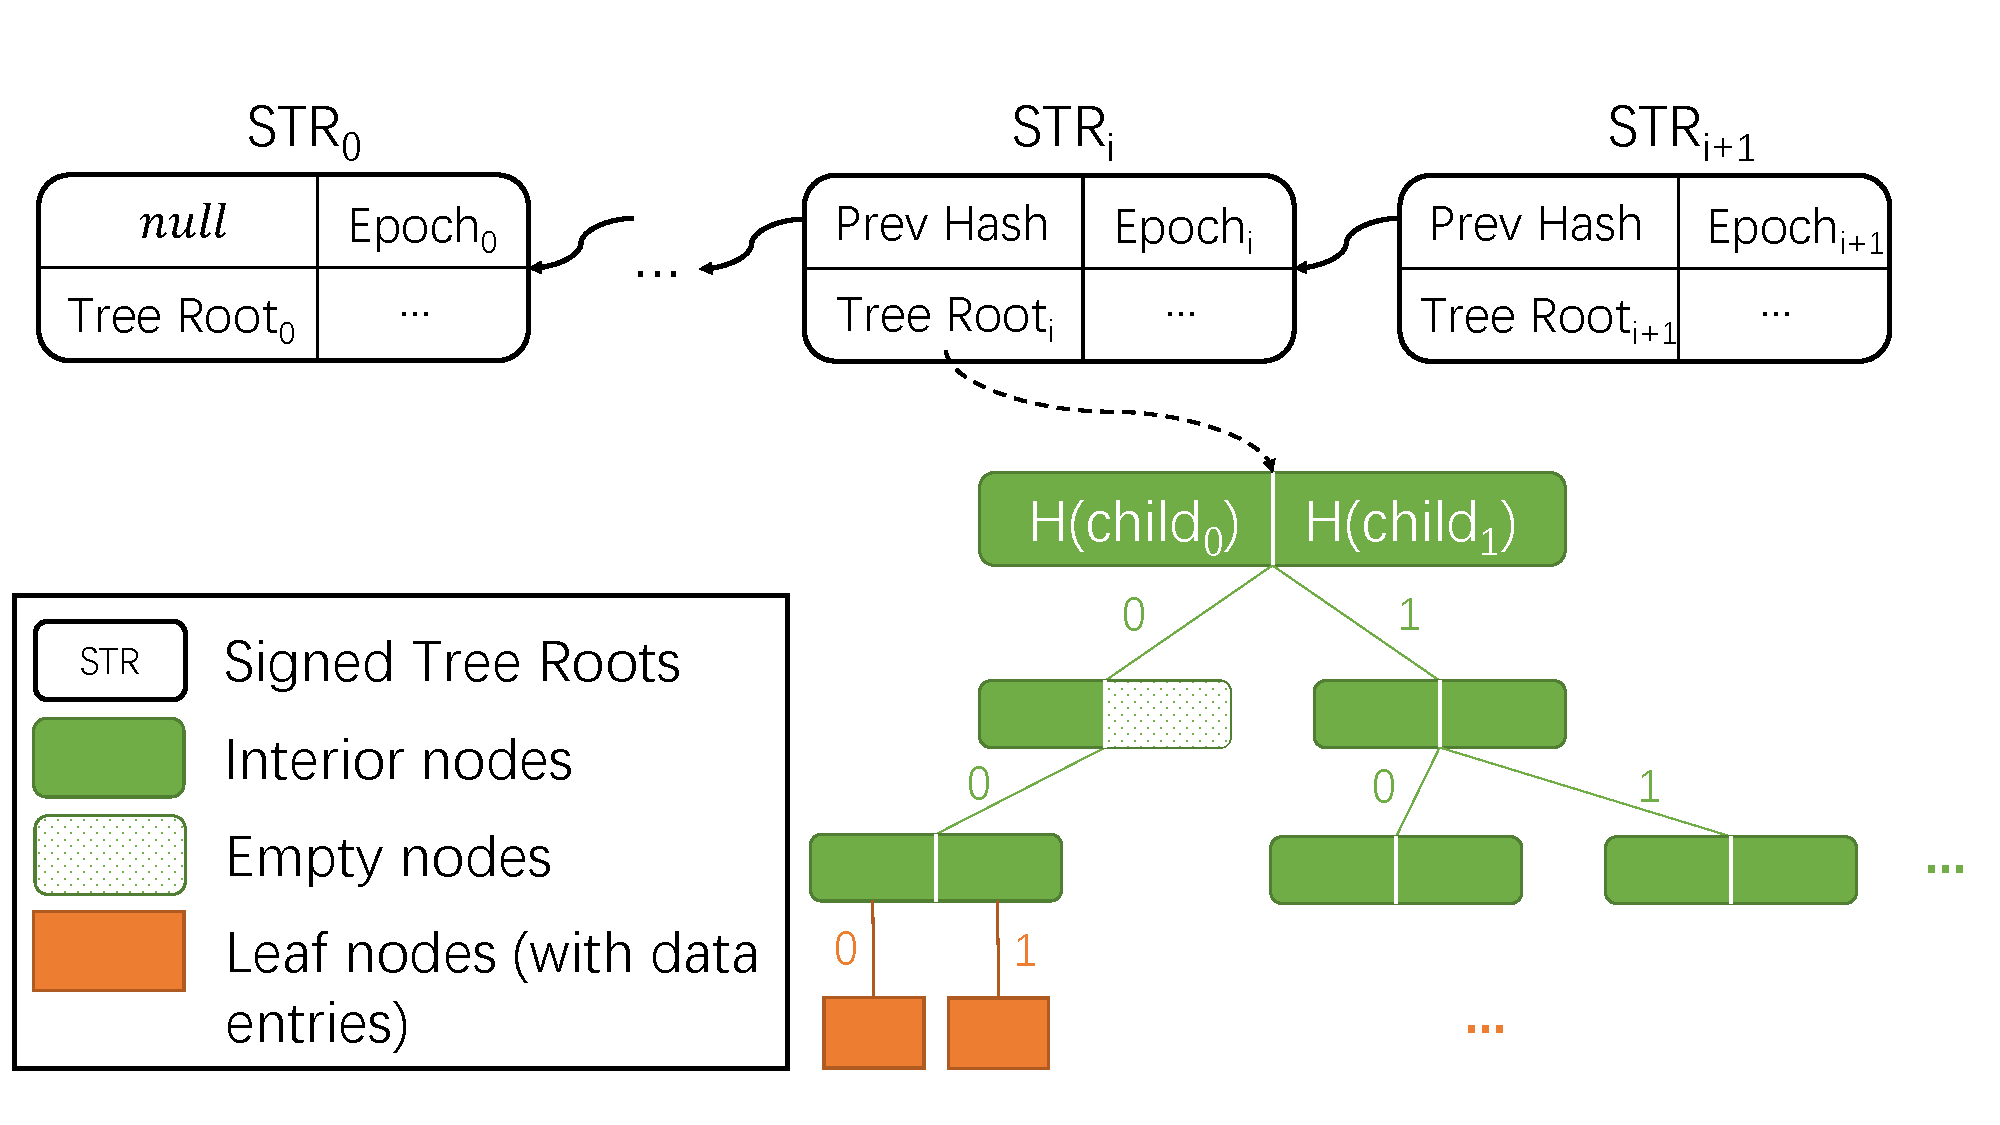
\includegraphics[height=4cm]{figs/arch_conkis.pdf}
        \caption{CONIKS architecture}
        \label{fig:conkis}
    \end{minipage}
    \begin{minipage}{0.48\textwidth}
        \centering
        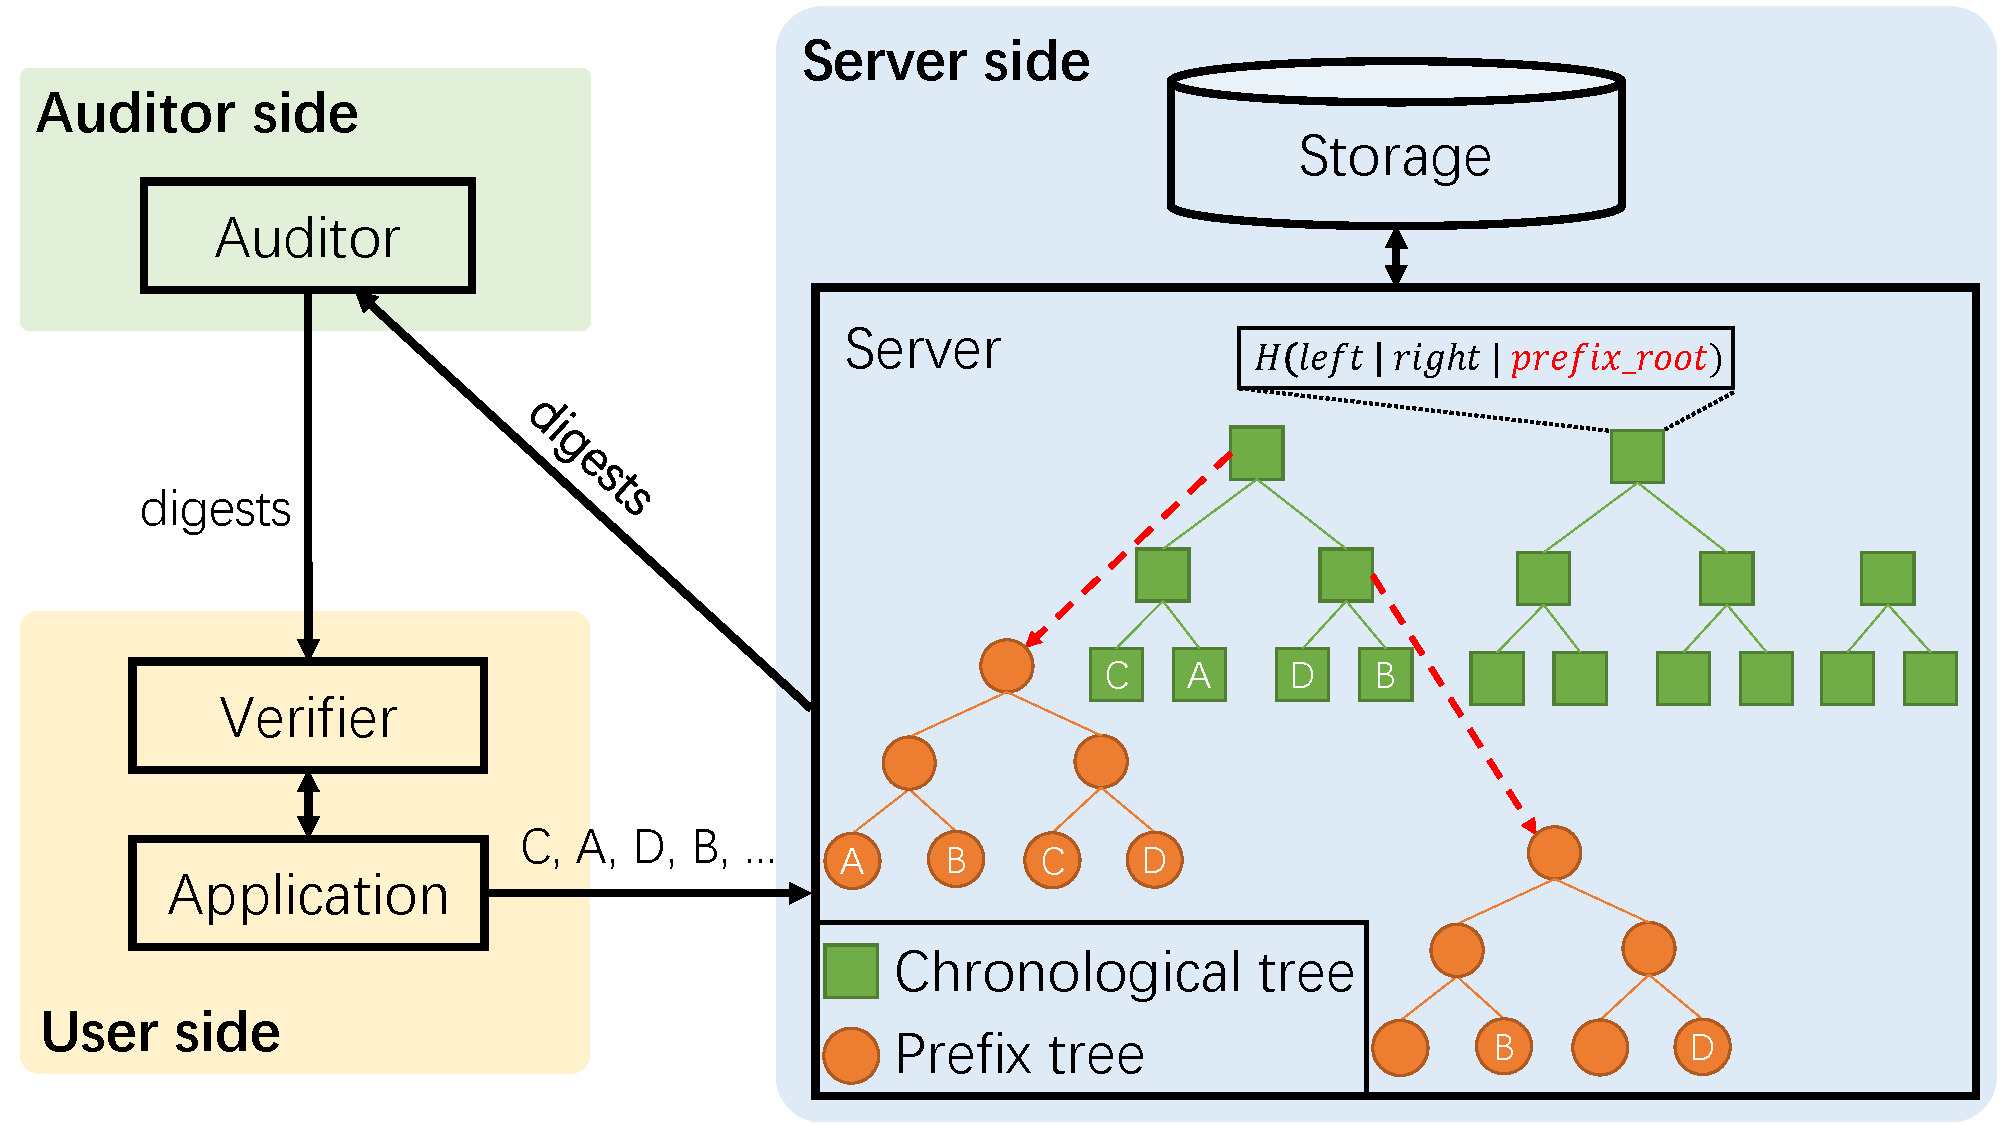
\includegraphics[height=4cm]{figs/arch_merkle2.pdf}
        \caption{Merkle$^2$ architecture}
        \label{fig:merkle2}
    \end{minipage}
\end{figure}

\section{Ledger Databases}
\label{sec:ldb}

In this section, we will describe the details of ledger databases and the design choices of existing systems.

\subsection{Threat Model}

Ledger databases adopt a threat model assuming that a single-party service provider can be malicious or compromised.
Users are only able to detect the malicious behaviors instead of preventing them. 
Many systems also rely on a group of trusted auditors to help verify the data integrity and notify the users of malicious behaviours, and therefore, relieve the burden on users.

\subsection{Ledger Structure}

Ledger is the key data structure of ledger databases. It maintains all current and historical data in an authenticated data structure (ADS), where proofs can be generated for verifying the data integrity. The ADS is usually a Merkle variance. For example, QLDB builds a Merkle tree over hashes of all data as shown in Figure~\ref{fig:qldb}. SQL Ledger constructs a Merkle tree over the modified data for each transaction, and another Merkle tree over the transaction entries batched in a block. The root hash of the latter Merkle tree is stored in the block entry with the previous block entry's hash to form a hashed chain as shown in Figure~\ref{fig:sqlledger}. LedgerDB adopts a batched accumulated Merkle tree, which adopts copy-on-write when new transactions are appended to reduce the contention as shown in Figure~\ref{fig:ledgerdb}. Trillian shown in Figure \ref{fig:trillian} adopts a sparse Merkle tree to store the data, therefore, it does not allow different versions of the same key. CONIKS stores the data in Merkle prefix trees, the root hashes of which are linked in a linear hash chain as shown in Figure \ref{fig:conkis}. To improve the efficiency of verification for the latest versions, Merkle$^2$ shown in Figure \ref{fig:merkle2} constructs a forest of full Merkle trees over data in chronological order, and each internal node contains the root hash of a prefix tree built over data in lexical order.

\subsubsection{Chronological order vs. lexical order}
Systems such as QLDB, LedgerDB, and SQL Ledger construct ADS over data in chronological or transaction order. The ADS is used only for integrity proof, and separate index structures are required to query the data. 
This causes two problems: 1) updating and proof generation become slower when the ADS grows larger; 2) It requires additional protection of the indexes, e.g., LedgerDB uses a Merkle Patricia Trie(ccMPT) to protect its clue indexes, while the index tables in QLDB and SQL Ledger are not hash protected, rendering its inability to guarantee that the value is the latest.
While systems like Trillian, CONIKS, and Merkle$^2$ embed additional Merkle variance in lexical order, which could serve as protected indexes of data.

\subsection{Query Processing}

\subsubsection{Abstraction}

Certificate transparency logs, for the purpose of storing keys and certificates, usually expose simple key-value store abstractions. While commercial ledger databases, which target on exchanging of assets or general business logic, support transaction with ACID properties. In particular, QLDB and LedgerDB directly build the ledger over the transaction logs. Alternatively, SQL Ledger commits the transaction to a separate transaction log for failure recovery, and creates the ledger at a later stage.

\subsubsection{Batching}
The update of the ledger is expensive since it involves calculating intensive cryptographic hashes and incurs high contention, especially for the root node, making it hard for parallelism. 
To reduce the hash calculation and mitigate the read/write contention against proof generation operations, LedgerDB updates its ADSs by batches of transactions and adopts copy-on-write when updating the ADSs. SQL Ledger constructs an individual Merkle tree for each transaction and block, making it contention-free when appending new blocks to the ledger. Similar to LedgerDB, SQL Ledger batches multiple transactions in a block to reduce the overhead of calculating block-level hashes.

\subsection{Verification}

To guarantee the integrity of data and query results, ledger databases provide proofs that can be publicly verified by the users or third-party verifiers for each request. 
The proofs of a ledger database typically consist of a digest which is a hash summary of the entire ledger structure, a proof containing the hashes of the Merkle tree nodes along the path from the root to the leaf node the data located. 
The client, upon receiving the proof, can reproduce the digest by calculating the hashes recursively. 
It then verifies the integrity of data by comparing the original and reproduced digest.

\subsubsection{Deferred verification}
It is expected that providing
%%% ooibc: such?
%%% so far from the previous argument
proof for each operation is costly. 
LedgerDB~\cite{ledgerdb} and SQL Ledger~\cite{sqlledger} adopt deferred verification. The system, on completion of the operation, will return a promise containing the data and block sequence the data resides to the users for future verification. The client can batch the proof generation request and verification process for higher performance. 
However, there is a trade-off between performance and security. There is a verification time window that the integrity of data could be temporarily violated.

\subsection{Auditing}
Systems such as certificate transparency, LedgerDB, and SQL Ledger rely on auditors to check the consistency of the ledger and detect malicious behaviors. The auditors will rebuild the ledger based on the logs and compare the digest of the rebuilt ledger and that requested from servers.
It will notify the users of the misbehavior if any mismatching is found. The auditing process is typically expensive. 
Any third-party entities or powerful users can play the role of the auditor. 
The systems require at least one honest auditor so that any malicious behaviours can be detected and notifications can be sent to the users. QLDB does not rely on auditors to check the consistency of the ledger. Consequently, users have to check the consistency of the ledger if required.


\section{Design}
\label{sec:design}

\subsection{Architecture}
\label{sec:overview}

\begin{figure}
    \centering
    \begin{minipage}{0.48\textwidth}
        \centering
        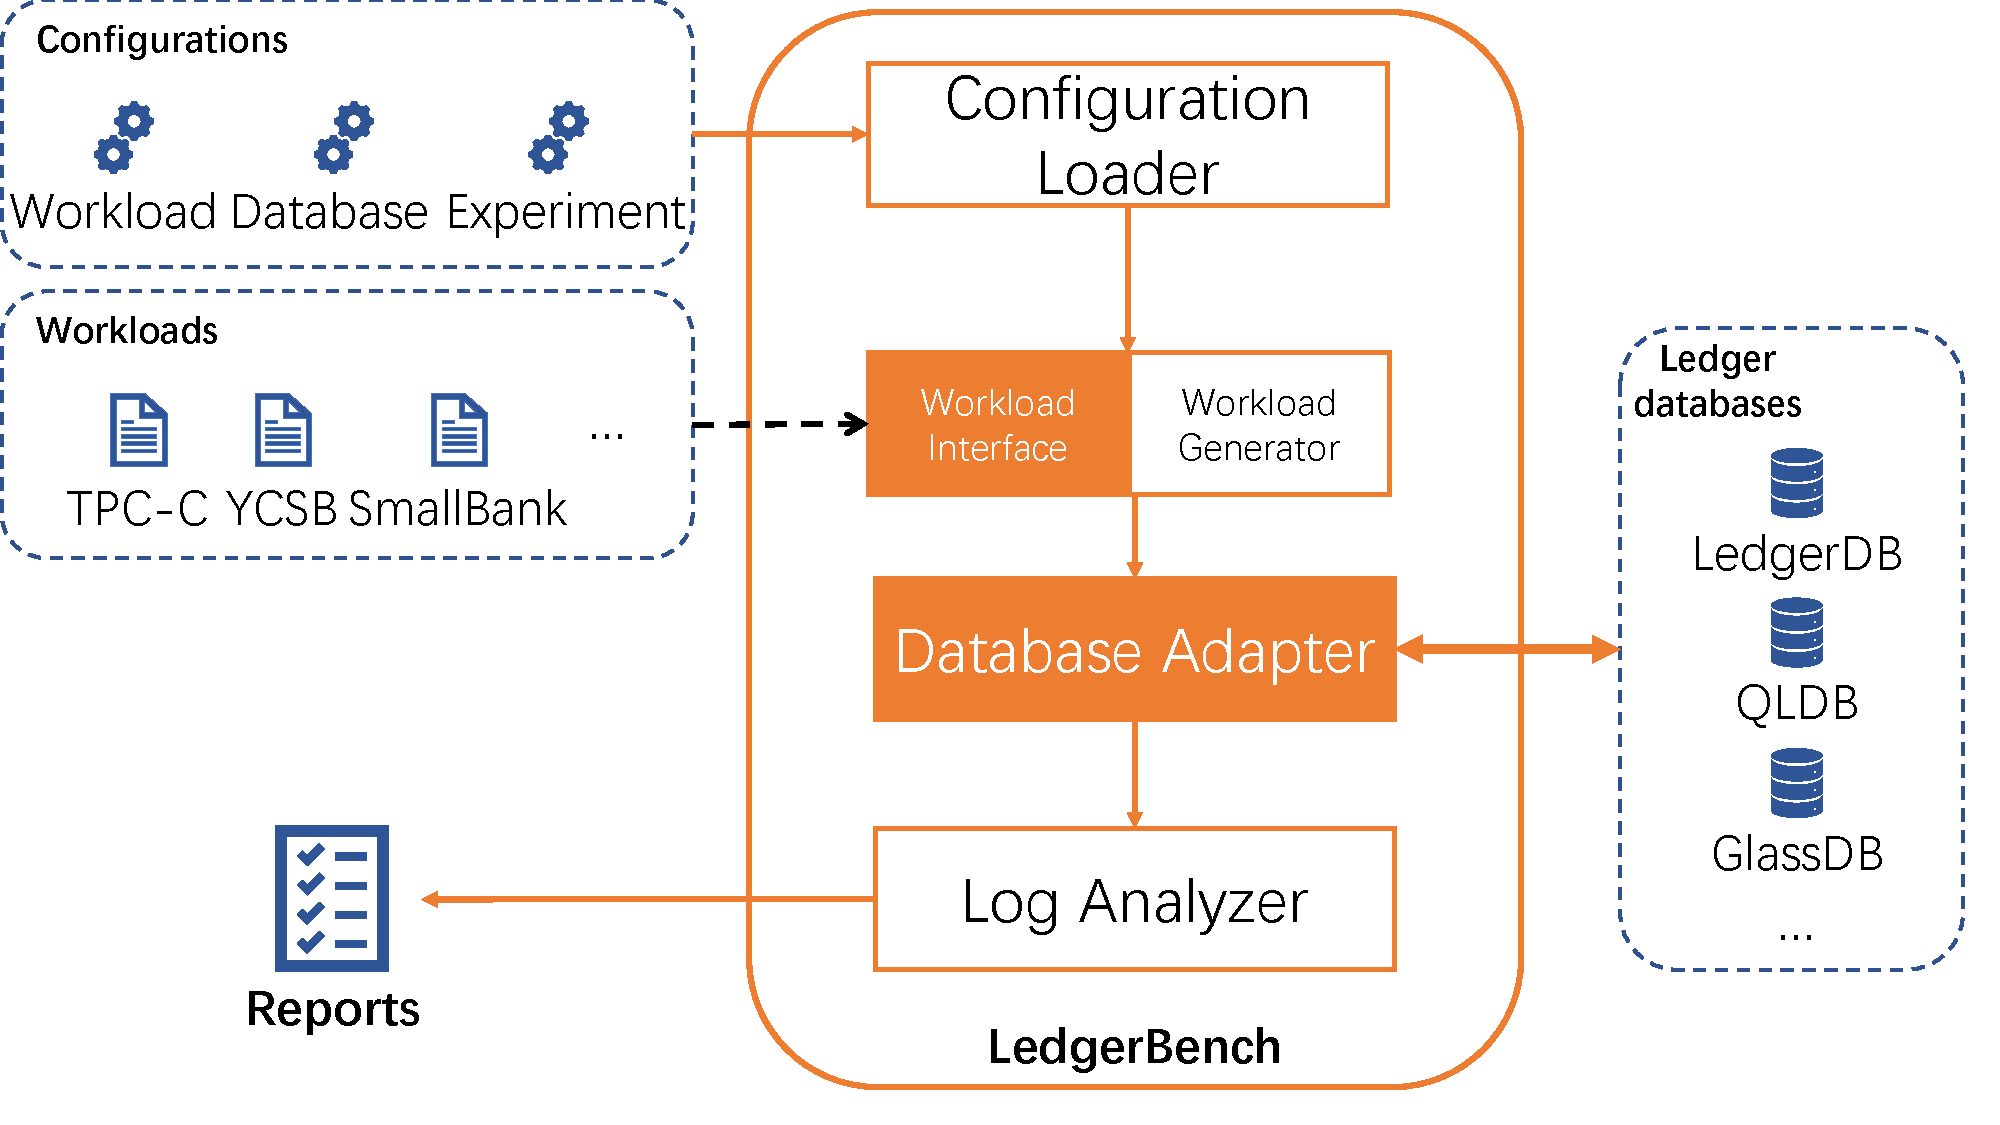
\includegraphics[height=4cm]{figs/arch_ledgerbench_fullsize.pdf}
        \caption{\systemname architecture}
        \label{fig:structure}
    \end{minipage}
    \begin{minipage}{0.48\textwidth}
        \centering
        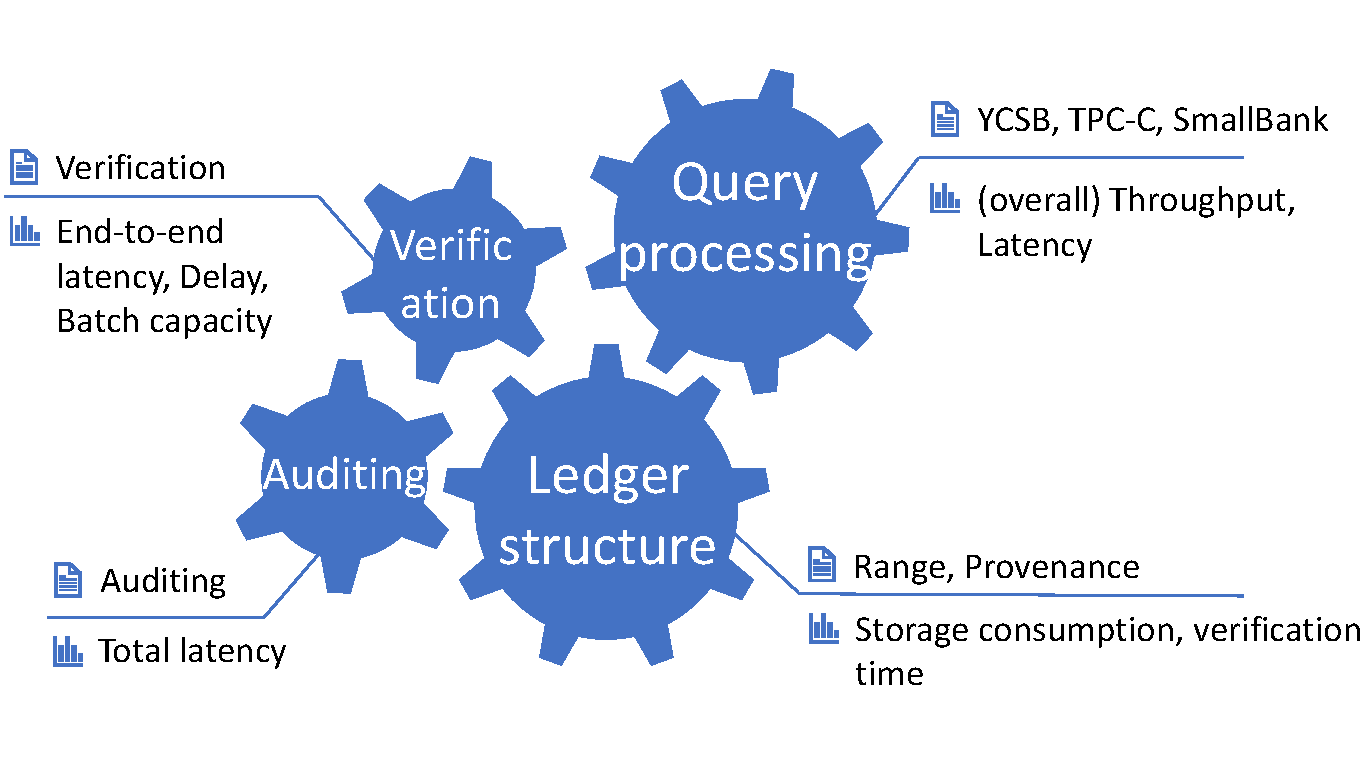
\includegraphics[height=4cm]{figs/abstraction-fullsize.pdf}
        \caption{Abstraction of ledger databases and the corresponding workloads and metrics of each component.}
        \label{fig:abstraction}
    \end{minipage}
\end{figure}

Figure~\ref{fig:structure} shows the architecture of \systemname. It contains a configuration loader, a workload generator, database adapters, and a log analyzer. 
The configuration loader loads the parameters of the benchmarks. The workload generator creates tasks by generating the operations and corresponding arguments based on the parameters. 
It sends the generated tasks to the database adapters through HTTP requests. The database adapters, on receiving the tasks, initialize database clients for execution. It logs the metrics collected, which are later processed by the log analyzer for final results.



\textbf{Configuration loader.} Configuration Loader is responsible for loading all experiment-related configurations at runtime. It reads the parameters from the command line and configuration files. The configurations include workload configurations, e.g., distribution of operations, database configurations, e.g., block time, and experiment configurations, e.g., number of testing threads, request rate, etc.

\textbf{Workload generator.} Workload generator issues the tasks to the database adapter via HTTP. According to the workload configuration, it creates the tasks consisting of the operation type and a list of parameters. 
Users can control the load by specifying in the experiment configurations the number of nodes and threads to run the workload generators and the request rate of each workload generator. The workload generator is implemented in a way that is easy to extend. It exposes a uniform workload interface, based on which a driver is implemented for each workload type. Users can add customized workloads by simply implementing the workload interface. 
Depending on the configuration, the workload generator initiates different drivers.
% zch: To sum up, the workload generator first generates instructions to start and initialize the database specified by database configurations and then fires tasks according to workload configurations.
%%% ooibc
%%% ???

\textbf{Database adapter.}
%Upon receiving the requests from the task generators, database adapters store the tasks in a queue, from which a pool of database clients, initialized in advance, can poll. Similarly, it is easy for users to extend new database systems to \systemname. 
%%% ooibc:
%%%% ????
Database adapter maintains a pool of database client instances, which connect to the ledger database being evaluated. Upon receiving the requests from the task generators, database adapters store the tasks in a queue, from which the client instances fetch tasks and send them to the database for execution. Similar to workload generator, it is easy for users to extend new database systems to \systemname as
it exposes a general interface for each workload operation. Users only need to implement the function with the database clients to be tested. Database adapters can be implemented in any programming language since the tasks are sent via HTTP.

\textbf{Log analyzer.} Measurements are taken and logged before and after the execution of the workload tasks. The log analyzer processes the logs and calculates the required metrics.

\subsection{API}
\label{subsec:api}

In this section, we describe the APIs of the workload generator and database adapter. Users are able to include customized workloads and ledger databases by simply inheriting the interfaces. First, we describe the API of the workload generator as follows.

\begin{itemize}
    \item \texttt{NextTask(conf).} The interface takes the workload configuration as input and generates the next task including the operation type and a list of parameters. The configuration usually contains the ratio, distribution, and ranges of operations, keys and values. For example, a configuration of Smallbank workload includes $D(operation) = uniform, D(account) = uniform, R(account) = [0, 100000], R(ammount) = [0,1000]$, where $D$ is the distribution, and $R$ is the range. The interface returns the generated tasks, e.g., $<SendPayment, 1, 2, 200>$, which represents account 1 paying $\$200$ to account 2.
\end{itemize}

Next, we introduce the APIs of the database adapter. Depending on the database under evaluation, the database adapter may be implemented in different programming languages.

\begin{itemize}
    \item \texttt{ExecuteTransaction(task, db).} The interface takes the task generated by \texttt{NextTask} and the database adapter, \texttt{db}, as the input and returns the status of execution. The inherit function implemented by the user shall execute the transaction with a sequence of \texttt{Put}, \texttt{Get}, and \texttt{Verify} operations provided by the database adapter.
    \item \texttt{Put(keys, values).} This interface defines the operation to update or insert a list of keys and values in the database. It will return the proof optionally for databases that do not support deferred verification.
    \item \texttt{Get(keys).} This interface defines the operation to get the values of a list of keys from the database. It will return the proof optionally for databases that do not support deferred verification.
    \item \texttt{Verify(keys, block\_seqs).} This interface is for deferred verification, where a batch of keys could be verified together. The input of the interface is a list of keys and block sequences the keys are located. The inherit function shall get the proofs from the database, verify the proofs, and return the verification result.
    \item \texttt{Verify(proof).} This interface is for immediate verification, where the input \texttt{proof} can be obtained from the \texttt{Get} and \texttt{Put} operations. The interface returns the verification result.
\end{itemize}

To extend \systemname with a new workload, users need to implement the \texttt{NextTask} and \texttt{TransactionX}. To include a new database for evaluation, users need to implement the \texttt{Put}, \texttt{Get}, and \texttt{Verify}. 

\subsection{Metrics}

\systemname evaluates ledger databases on their four components described in Section~\ref{sec:ldb}. Figure~\ref{fig:abstraction} shows the metrics with respect to each component. 
The query processing component is responsible for query execution and data commitment. It is critical to know how fast the system can process data. Therefore, we measure the system-level throughput and latency of running key-value or OLTP workloads.
While for ledger structures, the time- and space-efficiency of the access and verification methods are the key factors. Hence, the storage consumption and execution time of verification performed by the clients are taken as metrics.
To evaluate the verification performance, we take the end-to-end latency of user verification requests, the number of keys each verification request will process for a batched verification, and vary the delay time for a deferred verification.
Lastly, \systemname evaluates the auditing process by taking the latency of auditing a batch of transactions.


\subsection{Workloads}
\label{sec:workload}
In this section, we describe the workloads used in \systemname.
We include a verification-aware workload adapted from Smallbank.
We also implement range query workloads in addition to the point queries covered in Smallbank.
Users can easily extend \systemname with more workloads with the API described in Section \ref{subsec:api}.

\textbf{SmallBank.}
There are two tables in our SmallBank workload, namely saving and checking, to simulate bank services such as querying balances, depositing and transferring money, and amalgamating assets among 100,000 bank accounts. Similarly, we implement all the six transactions in the context of verifiable databases, i.e., each transaction will return the corresponding proof to verify the integrity of this execution.

\textbf{Range.}
To evaluate the effectiveness of indexing and block policies of a ledger database, we implement the range query workload. It queries a random range of keys. In our experiments, the queried keys follow a uniform distribution.  Besides the corresponding values, we also request a promise, which is used later to validate the integrity of the ledger.

%%% ooibc: HERE

\section{Evaluation}
\label{sec:exp}

In this section, we benchmark the state-of-the-art ledger databases, namely, QLDB, LedgerDB, and SQL Ledger. QLDB is a commercial product offered by Amazon. LedgerDB is an industrial prototype implemented by Alibaba. SQL Ledger is a commercial product provided by Microsoft.
We evaluate the systems with both macro-benchmarks and micro-benchmarks. Since there are no source codes for the systems, we re-implement the systems based on the online documentation and paper. We conduct the experiments on 24 machines equipped with 10$\times$2 Intel Xeon W-1290P processors, 128GB RAM, and 10 Gbps Ethernet. We start 16 server nodes and 8 client nodes. Each client node will run 20 client processes.

\subsection{Macro Benchmarks}

This section evaluates the performance of an end-to-end query processing with Smallbank, and range workloads.

\begin{figure}
    \begin{minipage}{0.48\textwidth}
        \centering
        \subfloat[Throughput]{
            \centering
            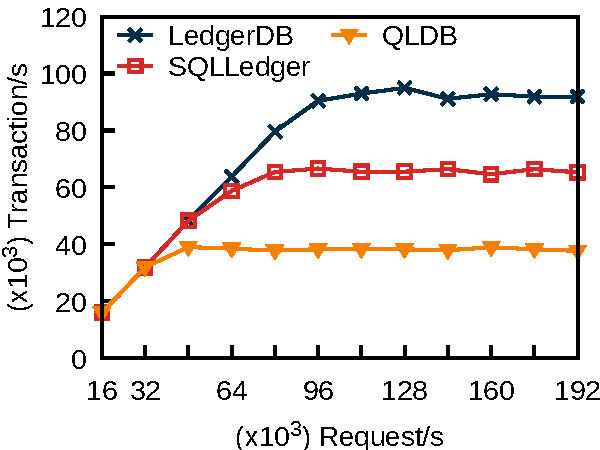
\includegraphics[height=3cm]{figs/smallbank_tps_client.pdf}
            \label{fig:exp:smallbank_lat}
        }
        \subfloat[Latency]{
            \centering
            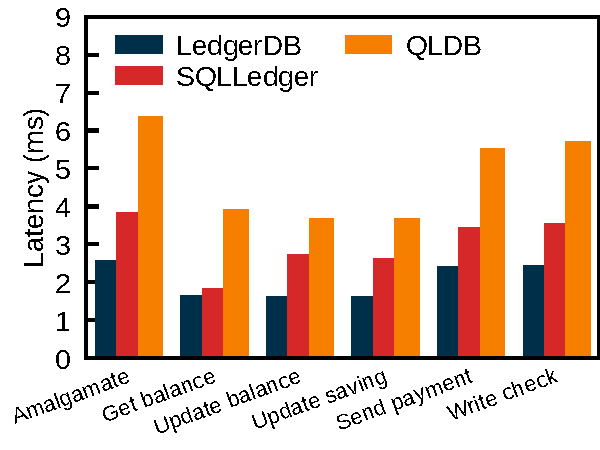
\includegraphics[height=3cm]{figs/smallbank_lat_op.pdf}
            \label{fig:exp:smallbank_tps}
        }
        \caption{Performance for Smallbank workloads}
    \end{minipage}
    \begin{minipage}{0.48\textwidth}
        \subfloat[Throughput]{
            \centering
            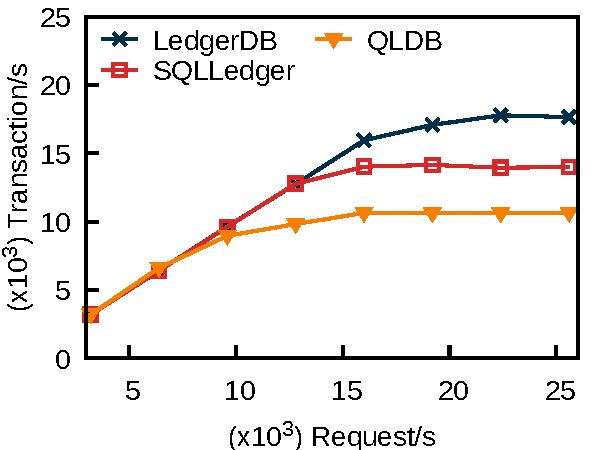
\includegraphics[height=3cm]{figs/range_tps.pdf}
            \label{fig:exp:range_tps}
        }
        \subfloat[Latency]{
            \centering
            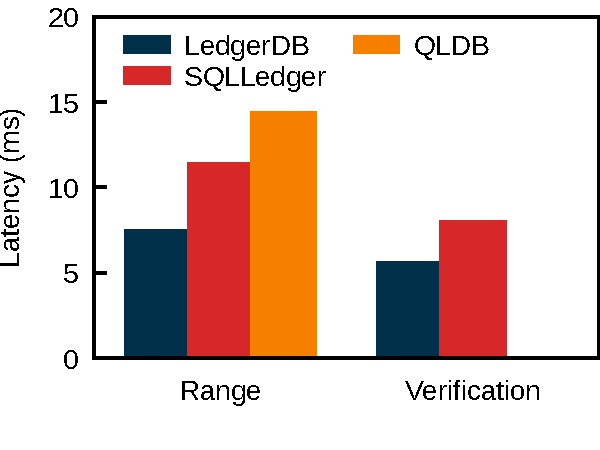
\includegraphics[height=3cm]{figs/range_lat.pdf}
            \label{fig:exp:range_lat}
        }
        \caption{Performance for range workload.}
        \label{fig:exp:range}
    \end{minipage}
\end{figure}


\subsubsection{Smallbank}

We initialize 100,000 users with 1000 dollars in their saving account and 50 dollars in their balance account. The experiment is conducted by feeding the system with transactions that consist of one of the six operations with equal probability. We first vary the total request rates from 16,000 to 192,000. Figure~\ref{fig:exp:smallbank_tps} shows the throughputs of the system with increasing client requests. LedgerDB outperforms SQL Ledger by up to $1.4\times$, and outperforms QLDB by $2.4\times$. LedgerDB and SQL Ledger outperform QLDB by adopting asynchronous ledger updates and deferred verification. In contrast, QLDB incurs significant overhead updating the ledger for each commit and performing verification after each operation. LedgerDB performs better than SQL Ledger because the clue indexes used to access the data are built over versions, and therefore, much smaller compared to the ledger and history table indexes in SQL Ledger. The heads of the clue indexes are stored in memory for executing queries efficiently. Figure~\ref{fig:exp:smallbank_lat} shows the average latency of specific operations. The results show similar trends that LedgerDB has the lowest latency, while QLDB has the highest latency.


\subsubsection{Range}

We conduct the experiment with a dataset consisting of 100,000 keys. 
The ranges are selected with random sizes from 10 keys to 20 keys. The results are depicted in Figure~\ref{fig:exp:range}. LedgerDB has the highest throughput. It builds a separate clue index for each key and requires scanning the head of all clue indexes when processing the range query. The overhead is mitigated since all clue index heads are stored in memory. SQL Ledger requires fetching additional metadata for future verification. The verification process is more costly due to the need of scanning the blocks. QLDB performs the worst as it verifies the data after each operation.


\subsection{Micro Benchmarks}

In this section, we evaluate each component of the systems with micro-benchmarks. 

\subsubsection{Verification}


We evaluate the execution time and proof size for verifying one key from the client side, and show the results in Figure~\ref{fig:exp:verify}. LedgerDB has the highest proof size and verification time. This is because the verification of clue indexes is expensive. In particular, users need to verify the ccMPT to validate the number of entries stored in the clue index, and then verify each entry on the ledger. Though such tasks can be delegated to the auditors, users cannot guarantee the clue indexes are not tampered with after the auditing process. The proof sizes of QLDB and SQL Ledger are small, since they only contain a list of hashes on a path of the Merkle tree. However, QLDB and SQL Ledger fail to guarantee that the fetched data is the latest.


\subsubsection{Delay}

\begin{figure}
    \centering
    \begin{minipage}{0.24\textwidth}
        \centering
        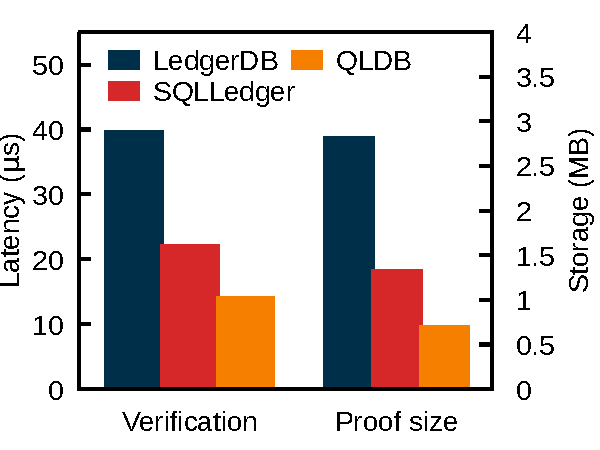
\includegraphics[height=3cm]{figs/micro_verification.pdf}
        \caption{Verification latency and proof size.}
        \label{fig:exp:verify}
    \end{minipage}
    \begin{minipage}{0.24\textwidth}
        \centering
        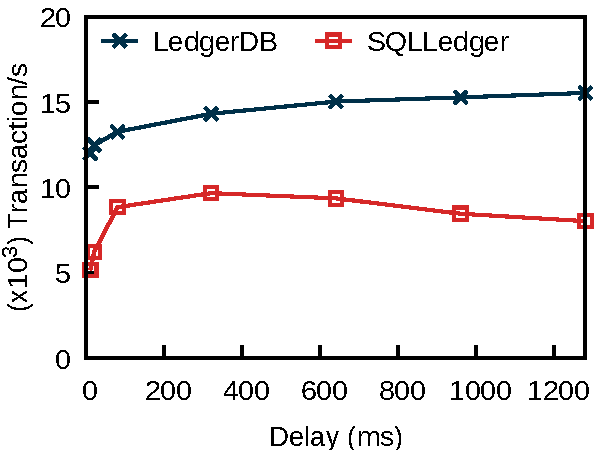
\includegraphics[height=3cm]{figs/micro_delay.pdf}
        \caption{Performance with delay setting.}
        \label{fig:exp:delay}
    \end{minipage}
    \begin{minipage}{0.24\textwidth}
        \centering
        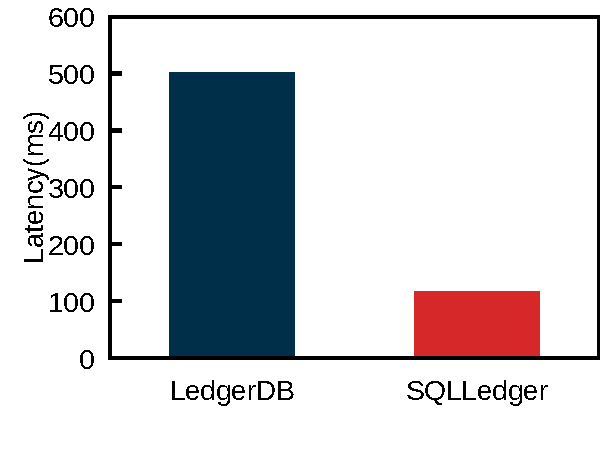
\includegraphics[height=3cm]{figs/micro_audit.pdf}
        \caption{Latency for auditing one block.}
        \label{fig:exp:audit}
    \end{minipage}
    \begin{minipage}{0.24\textwidth}
        \centering
        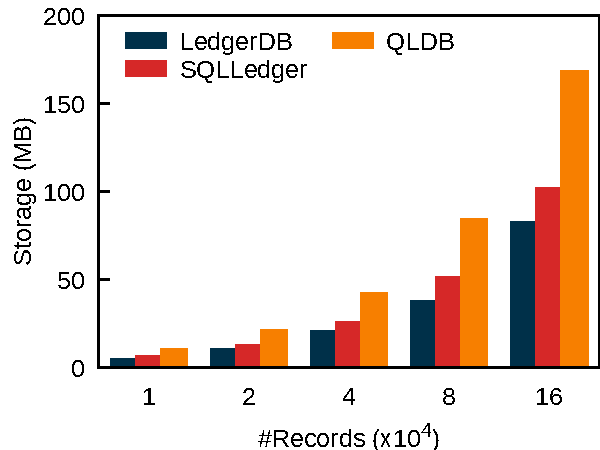
\includegraphics[height=3cm]{figs/micro_storage.pdf}
        \caption{Storage consumption.}
        \label{fig:exp:storage}
    \end{minipage}
\end{figure}

In this section, we evaluate how delay time affects the performance. We use a range of delay time from 10ms to 1280ms, and depict results in Figure~\ref{fig:exp:delay}. We can observe that the performance of all systems increases as the delay time increases in the beginning. This is because a higher delay time will result in a larger verification batch, which allows the servers to provide more efficient batched proof. As the delay time keeps increasing, the performance will drop because the overwhelming data cause significant overhead and high contention when generating the proofs.

\subsubsection{Audit}

This section evaluates the cost of the auditing process for LedgerDB and SQL Ledger. We start with 16 server nodes and 8 client nodes with each client node running 20 client processes. We feed all clients with a read-write key-value workload. Then we start an audit client executing audit tasks every second.
To fairly compare the two systems, we set the block time of both systems to be 10ms, i.e., all transactions within the period are collected to a block and appended to the ledger. The auditor will verify the block of transactions for each auditing request.
Figure~\ref{fig:exp:audit} shows the average latency for auditing one block. Both systems batch around 700 transactions in a block. The latency of LedgerDB is $4\times$ the latency of SQL Ledger. This is because verification for clue indexes is expensive in LedgerDB. Note that SQL Ledger does not verify its ledger table and history table, therefore, the integrity of data cannot be fully guaranteed. Though the queried data can be verified using the proof generated from the ledger, the system can always return stale data and still pass the verification. 

\subsubsection{Storage}

We measure the storage consumption of the systems with respect to the total number of records stored in the systems, from 10,000 to 160,000. LedgerDB and SQL Ledger adopt transaction batching and update the ledger less frequently, and are therefore more space-efficient than QLDB. SQL Ledger consumes slightly more storage compared with LedgerDB because of the additional indexes.

\section{Related Works}
\label{sec:related}

Existing works have been done to explore the opportunity of fusion designs of blockchain and database \cite{bc&ddbms,provenance, veritas, bigchaindb, blockchaindb, hybridblockchain, bcbook, untanglingbc}.
% todo: summary
However, the systems above try to enable database's query ability on top of blockchains, therefore suffering from the low performance of blockchains. While the ledger databases \cite{qldb, ledgerdb, sqlledger} use the ledger structures similar to the blockchain and build verifiable database with a central party, therefore, are more practical in processing OLTP workloads. Spitz \cite{spitz} proposes to integrate a ledger in the HTAP system. This work focuses more on evaluating the ledger databases and their designs, though it can also be used to evaluate blockchains.

There are many existing benchmark frameworks. BlockBench \cite{blockbench} is the first framework to comprehensively evaluate the private blockchains from the application layer, execution engine, data model and consensus. Hyperledger Caliper \cite{caliper} is another widely-used blockchain benchmark tool, supporting a range of systems such as Hyperledger Fabric \cite{hyperledger}, Ethereum \cite{ethereum}, Fisco-Bcos \cite{fisco}, etc.
OLTP-Bench \cite{oltpbench} and YCSB \cite{ycsb} are benchmarking tools for relational database and key-value store, respectively.
While \systemname focuses on the ledger database specific designs to evaluate the systems in every aspect.


\section{Conclusions}
With the increasing digitization of businesses and cloud hosting, there have been increasing demands for transactions to be verifiable and auditable.
Various commercial ledger databases have been designed to meet the demands by supporting the integrity of data, history and query results. 
We conduct a survey on the designs of some existing systems. We examine the design of
these representative ledger databases,  identify four major components and discuss the design choices of each component. 
We then outline LEDGERBENCH, a framework for benchmarking ledger databases, for both macro-
and micro-benchmarking.
We conduct extensive performance study and identify various bottlenecks and their possible causes.  We hope the study and open source of the framework will facilitate further development in this important area.

\label{sec:conclusion}

\begin{thebibliography}{10}
\itemsep=1pt
\begin{small}

\bibitem{hyperledger} Elli Androulaki, Artem Barger, Vita Bortnikov, Christian Cachin, Konstantinos Christidis, Angelo De Caro, David Enyeart, Christopher Ferris, Gennady Laventman, Yacov Manevich, et al. 2018. Hyperledger fabric: a distributed operating system for permissioned blockchains. In EuroSys. 30.

\bibitem{ethereum} Gavin Wood et al . 2014. Ethereum: A secure decentralised generalised transaction ledger. Ethereum project yellow paper 151, 2014 (2014), 1–32.

\bibitem{quorum} ConsenSys. 2020. ConsenSys/quorum: A permissioned implementation of Ethereum supporting data privacy. https://github.com/ConsenSys/quorum.

\bibitem{ct} Google. 2020. Certificate Transparency. https://www.certificate-transparency.org/.

\bibitem{trillian} Google. 2020. Trillian: general transparency. https://github.com/google/trillian.

\bibitem{coniks} Marcela S. Melara, Aaron Blankstein, Joseph Bonneau, Edward W. Felten, and Michael J. Freedman. 2015. CONIKS: Bringing Key Transparency to End Users. In Usenix Security.

\bibitem{merkle2} Yuncong Hu, Kian Hooshmand, Harika Kalidhindi, Seung Jin Yang, Raluca Ada Popa. 2021. Merkle$^2$: A Low-Latency Transparency Log System. In IEEE Symposium on Security and Privacy.

\bibitem{ect} Mark D. Ryan. 2014. Enhanced Certificate Transparency and End-to-End Encrypted Mail. In NDSS.

\bibitem{qldb} Amazon. 2019. Amazon Quantum Ledger Database. https://aws.amazon.com/qldb/.

\bibitem{ledgerdb} Xinying Yang, Yuan Zhang, Sheng Wang, Benquan Yu, Feifei Li, Yize Li, and Wenyuan Yan. 2020. LedgerDB: A Centralized Ledger Database for Universal Audit and Verification. PVLDB.

\bibitem{sqlledger} Panagiotis Antonopoulos, Raghav Kaushik, Hanuma Kodavalla, Sergio Rosales Aceves, Reilly Wong, Jason Anderson, Jakub Szymaszek. 2021. SQL Ledger: Cryptographically Verifiable Data in Azure SQL Database. In SIGMOD.

% \bibitem{scaling} Kyle Croman, Christian Decker, Ittay Eyal, Adem Efe Gencer, Ari Juels, Ahmed E. Kosba, Andrew Miller, Prateek Saxena, Elaine Shi, Emin Gün Sirer, Dawn Song, and Roger Wattenhofer. 2016. On scaling decentralized blockchains. In Proc. 3rd Workshop on Bitcoin and Blockchain Research.

\bibitem{blockbench} Tien Tuan Anh Dinh, Ji Wang, Gang Chen, Rui Liu, Beng Chin Ooi, and Kian-Lee Tan. 2017. BLOCKBENCH: A Framework for Analyzing Private Blockchains. In SIGMOD.

% \bibitem{propagation} Christian Decker and Roger Wattenhofer. Information propagation in bitcoin network. 2013. In P2P.

% \bibitem{consistency} Eleftherios Kokoris-Kogias, Philipp Jovanovic, Nicolas Gailly, Ismail Khoffi, Linus Gasser, and Bryan Ford. Enhancing bitcoin security and performance with strong consistency via collective signing. 2016. In USENIX Security.

% \bibitem{shardprotocol} Loi Luu, Viswesh Narayanan, Chaodong Zheng, Kunal Baweja, Seth Gilbert, and Prateek Saxena. A secure sharding protocol for open blockchains. 2016. In CCS.

% \bibitem{bitcoinng} Ittay Eyal, Adem Efe Gencer, Emin Gün Sirer, and Robbert van Renesse. 2016. Bitcoin-ng: A scalable blockchain protocol. In NSDI.

\bibitem{caliper} Hyperledger foundation. 2018. https://www.hyperledger.org/use/caliper.

\bibitem{spitz} Meihui Zhang, Zhongle Xie, Cong Yue, and Ziyue Zhong. 2020. Spitz: a verifiable database system. PVLDB.

\bibitem{bc&ddbms} Pingcheng Ruan, Tien Tuan Anh Dinh, Dumitrel Loghin, Meihui Zhang, Gang Chen, Qian Lin, and Beng Chin Ooi. 2021. Blockchains vs. Distributed Databases: Dichotomy and Fusion. In SIGMOD.

\bibitem{provenance} Pingcheng Ruan, Gang Chen, Tien Tuan Anh Dinh, Qian Lin, Beng Chin Ooi, and Meihui Zhang. 2019. Fine-grained, secure and efficient data provenance on blockchain systems. PVLDB.

\bibitem{veritas} Johannes Gehrke, Lindsay Allen, Panagiotis Antonopoulos, Arvind Arasu, Joachim Hammer, Jim Hunter, Raghav Kaushik, Donald Kossmann, Ravishankar Ramamurthy, Srinath T. V. Setty, Jakub Szymaszek, Alexander van Renen, Jonathan Lee, Ramarathnam Venkatesan.2019. Veritas: Shared Verifiable Databases and Tables in the Cloud. CIDR.

\bibitem{bigchaindb} Trent McConaghy, Rodolphe Marques, Andreas Müller, Dimitri De Jonghe, Troy McConaghy, Greg McMullen, Ryan Henderson, Sylvain Bellemare, Alberto Granzotto. 2016. Bigchaindb: a scalable blockchain database. white paper, BigChainDB.

\bibitem{blockchaindb} Muhammad El-Hindi, Carsten Binnig, Arvind Arasu, Donald Kossmann, and Ravi Ramamurthy. 2019. BlockchainDB: a shared database on blockchains. PVLDB.

\bibitem{hybridblockchain} Zerui Ge, Dumitrel Loghin, Beng Chin Ooi, Pingcheng Ruan, and Tianwen Wang. 2022. Hybrid blockchain database systems: design and performance. PVLDB.

\bibitem{bcbook} Pingcheng Ruan, Tien Tuan Anh Dinh, Dumitrel Loghin, Meihui Zhang, Gang Chen. 2022. Blockchains: Decentralized and Verifiable Data Systems. Preprint.

\bibitem{untanglingbc} Tien Tuan Anh Dinh, Rui Liu, Meihui Zhang, Gang Chen, Beng Chin Ooi and Ji Wang. 2017. "Untangling Blockchain: A Data Processing View of Blockchain Systems," in TKDE.

\bibitem{pbft} Miguel Castro, Barbara Liskov. 1999. Practical byzantine fault tolerance. In OsDI.

\bibitem{credb} Kai Mast, Lequn Chen, Emin Gün Sirer. 2018. Enabling strong database integrity using trusted execution environments. arXiv preprint arXiv:1801.01618.

\bibitem{fisco} FISCO BCOS. The Building Block of Open Consortium Chain. https://www.fisco-bcos.org/

\bibitem{oltpbench} Djellel Eddine Difallah, Andrew Pavlo, Carlo Curino, and Philippe Cudre-Mauroux. 2013. OLTP-Bench: an extensible testbed for benchmarking relational databases. PVLDB.

\bibitem{ycsb} Brian Cooper, Adam Silberstein, Erwin Tam, Raghu Ramakrishnan, Russell Sears. 2010. Benchmarking cloud serving systems with YCSB. In SoCC.

\end{small}
\end{thebibliography}

\end{document}
